\chapter{\docname}
\label{\docname}
Dieses Kapitel beschreibt im Detail wie die Diplomarbeit gestaltet und abgegrenzt ist. Die Abgrenzung der Arbeit ist entscheidend wegen der hohen Komplexität des Projektes. Sie erfolgt durch Ziele, nicht-Ziele und optionale Ziele. Das ist im Unterkapitel 2.1 genau verfasst. 
Weiter folgt die Planung im Kapitel 2.3. Es werden hier das Lösungskonzept und die Projektmanagement erklärt. Es wird nun spezifiziert welche Projektmanagementmethode eingesetzt wurde.
\section{Projektziele}
In diesem Abschnitt werden die Ziele, nicht Ziele und optionalen Ziele beschrieben.
\subsection{Ziele}
Ziele sind wesentlich für jedes Projekt. Deshalb wurden die Ziele dieses Projekts in drei Kategorien geteilt.
In der ersten Kategorie gehören Ziele, die unbedingt erfüllt werden müssen. Anderfalls wurde das Projekt scheitern.
\begin{enumerate}
	\item Live vs. Foto unterscheiden.
	(3-dimensionale Erkennung an Gesicht machen. Tiefe messen damit zwischen einer Person und einem Foto differiert wird.)
	
	\item Gesichts-Schlüsselpunkt-Extraktion, um ein Gesicht zu identifizieren.
	
	\item Größe und Form der Augenhöhlen, Nase, Wangenknochen und Kiefer analysieren.
	
	\item Position/Verhältnisse der Hauptmerkmale relativ zueinander herausholen.
	
	\item Bilderdaten in Vektoren umwandeln mithilfe eines Algorithmus.
	
	\item Abstimmung (Vergleichen mit den Gesichtspunkten aller Personen in der Datenbank, um zu sehen, ob die Person schon registriert wurde).
	
	\item Bis zu 500 Personen in einer Datenbank speichern.
	
	\item 10 Tests, jeder Test in einer anderen Raumkondition, um m\"oglichst viele Betriebskonditionen zu testen.
	
	\item Datenbankdesign(Struktur der Datenbank, Datenbank erstellen, Datenbank einrichten)
	
	\item Error checking (\"Uberpr\"ufen, ob Fehler w\"ahrend des Betriebs auftreten)
	
	\item Safe Mode (eine Batterie, Back-ups in einem lokalen Server)
	
	\item Min. Arbeitsvorbereitung (Min. Gesichtsdetektionszeit)
	\item Admin account erstellen
	
\end{enumerate}
\subsection{Nicht Ziele}
%\newcommand{\autor}{Aron Terzeta}
Hier sind die Nicht-Ziele definiert, damit das Projekt begrenzt ist und damit Nichts gemacht wird, was nicht angefordert war.

\begin{enumerate}
	\item Mehr als ein Gesicht gleichzeitig erkennen.
	
	\item Maske, Brille oder Hüte w\"ahrend der Gesichtsdetektion tragen.
	
	\item Gesicht in Bewegung erkennen.
	
	\item Person ins Profil oder andere Position sein.
	
	\item Thermische Kamera einsetzen.
	
	
\end{enumerate}
\subsection{Optionale Ziele}
%\newcommand{\autor}{Jordi Zmiani}
Hier gehören Ziele, die optional sind. Das heißt sie sind nicht zwingend und wurden eingesetzt nur nachdem alle wichtigen und primären Ziele erfüllt sind.

\begin{enumerate}
	
	
	\item Öffnung der Haustüren oder jeder anderen Tür mit Gesichtserkennung.
	
	\item LCD-Display Implementation.
	
	\item Licht neben der Kamera (Night Vision implementieren damit die Erkennung/Registrierung auch dann funktioniert, wenn es dunkel ist.)
\end{enumerate}

\section{Projektplanung}

	Unsere Big Picture\footnote{vermittelt ein \"Uberblick \"uber das gesamte System.\cite{Bigpicture}} ist unser erstes grobes Design, das die Lösungsskizze des Projekts beschreibt. Es gibt bestimmte Gründe, warum Big Picture und Structed Design verwendet wurden, um die Software zu beschreiben. Diese Methode ermöglicht eine sehr gute Darstellung und Beschreibung des Lösungswegs. Ist schnell und leicht zu machbar. Alles ist klar sichtbar und nicht kompliziert. Big Picture und Structed Design\footnote{ist eine grafische Veranschaulichung des gesamten Systems. Das bedeutet, es wird wie bei einer Zwiebelschale mit der \"au{\ss}ersten Schicht begonnen. Jede weitere Schicht der Zwiebel geht weiter ins Detail.\cite{Bigpicture}} folgen dem Top-Down Prinzip, das heißt die Funktionen werden hierarchisch zerlegt (Jede Funktion wird in die folgenden Ebenen detaillierter beschreibt). Structed Design und Big Picture haben keine Begrenzung. Dort können eindeutig alle Funktionen, Schnittstellen, Signalen und Daten beschreibt werden, sodass es von allen leicht zu verstehen ist. Sehen Sie Abb. \ref{fig:bigpicture} 
	Unten wird die Legende auf Abb. \ref{fig:structed}.

\begin{figure}[ht]
	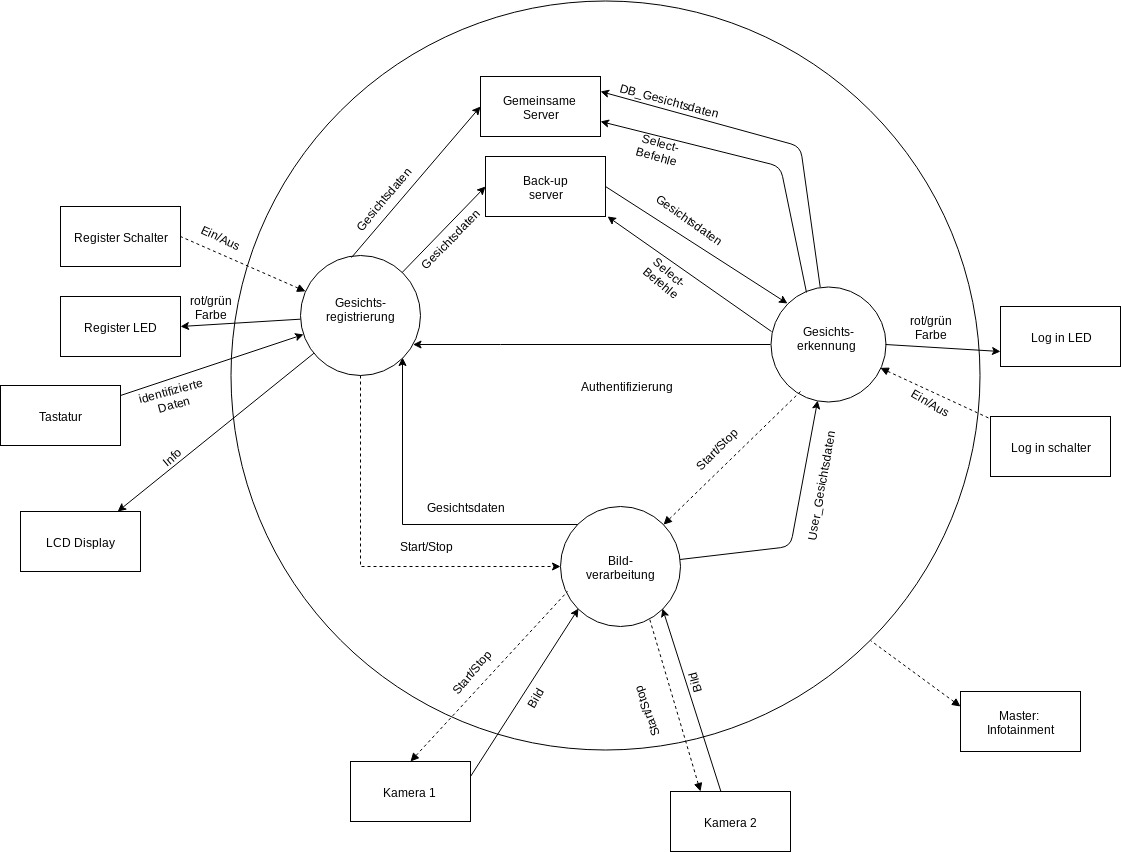
\includegraphics[width=0.8\textwidth]{./figures/Big_Picture.jpg}
	\centering
	\caption{Big picture}
	\label{fig:bigpicture}
\end{figure}
	\begin{figure}[ht]
	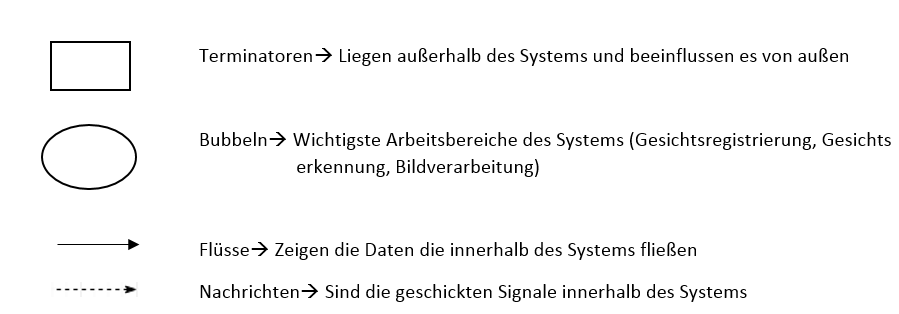
\includegraphics[width=0.8\textwidth]{./figures/Erklaerung_Erste_Ebene.png}
	\centering
	\caption{Legende: Structed Design}
	\label{fig:structed}
\end{figure}

\section{Projektmanagmentmethode}
Als Projektplanmethode haben wir Scrum, eine agile Methode, gewählt, weil es die Möglichkeit bietet, komplexe Projekte mit einem kleinen Personenkreis zu verwalten. Scrum ist ideal für Software- bzw. Hardware-Entwicklungsteams, weil das Team während des Projekts verschiedene Änderungen an seinem Plan vornehmen muss. Aus diesem Grund ist es besser, tägliche Zielvorgaben zu haben und in einem kurzen Zeitraum von 1 bis 4 Wochen so genannte Sprints durchzuführen, bei denen das Ziel am Ende dieser Springs ein Prototyp ist. Verschiedene Prototypen herzustellen und am Ende den richtigen auszuwählen, ist die beste Wahl für die Projektmanagementmethode zur Gesichtserkennung. Es gibt auch tägliche Pläne, in denen sich das Team zusammensetzt und entscheidet, was die Ziele für den Tag sind und was sie tun müssen.\cite{scrum}